\chapter{Knowledge-Based Communication}
\label{chap:improve}

Based on findings from previous studies, tools do not always effectively communicating with developers.
One reason this occurs is because of differences between developer knowledge and the information provided by notifications~\cite{johnson2016cross}.
Perhaps if tools could ascertain how much developers know about the concepts present in the information they provide, tools could provide feedback to better support developers in understanding and resolving defects.
The previous chapter suggested the ability to use developer source code contributions to predict how much they know about the concepts in tool notifications.

\textit{Given the ability to classify developers based on their knowledge of programming concepts, I propose improving the communication between tools and developers by providing knowledge-based notifications.}
Knowledge-based notifications would present information to developers based on how much they know about the concepts relevant to the defect.
To my knowledge, there are no existing studies that have explored adapting the information provided by tool notifications.

Despite notification adaptation being a new research area, adaptive user environments are becoming pervasive in research and practice~\cite{zou2008adapting, amershi2007unsupervised, stamper2009unsupervised}. 
Adaptive User Interfaces (AUI) use the experiences of users to adapt to better support the user.
Most relevant to this research are the models proposed by Zou and colleagues for adaptive menus in Eclipse~\cite{zou2008adapting}.
Similarly, this research explores using source code and machine learning to predict user knowledge but for adaptive tool notifications.


In this chapter, I discuss research that explores possible notification adaptations and the ability to improve communication by improving the support provided by tools to fill knowledge gaps and match developer expectations. 
To evaluate this proposal, I borrowed from existing research on expertise and problem solving to determine potential notification adaptations to evaluate and how they map to expertise.
I used the same concepts used in previous chapters to create and evaluate knowledge models: variables, exception handling, and generics.
I found notifications that communicate primarily about various aspect of these concepts, focusing on notifications that communicate about defects that are found in real software projects~\cite{ayewah2007evaluating, zheng2006value}.

I conducted 14 user studies with students and professional developers with various backgrounds and knowledge regarding the concepts of interest to evaluate their ability to resolve notifications designed for their level of expertise. This study was designed to evaluate the following hypotheses and research question:
\begin{itemize}
    \item [H\textsubscript{1}] Knowledge-based notifications can decrease the time required for notification resolution.
    \item [H\textsubscript{2}] Knowledge-based notifications increase developer likelihood of resolving notifications. 
    \item [H\textsubscript{3}] Knowledge-based notifications decrease developer attempts to resolve notifications.
    \item[RQ] Do developer adaptation preferences match expectations, based on existing literature?
\end{itemize}


\section{Proposed Approach}

For adaptive tool notifications to be realized, it is necessary to determine how tools should present information to developers. Previous research suggests one thing to consider when presenting information regarding a defect is the knowledge of the developer~\cite{johnson2016cross}.
To evaluate H\textsubscript{1} -- H\textsubscript{3}, I conducted user studies where I presented developers with adapted notifications and asked them to resolve each. In this section, I will outline the related research I used to create the adapted notifications and the approach I used to evaluate notification adaptations.

\subsection{Notification Adaptations}

Existing research on notification design focuses on the general information needs of all developers, regardless of their knowledge regarding the notification or its concepts~\cite{smith2015questions, barik14, robillard2014recommendation}. Therefore, there is no existing work that has examined notification design for expertise. 

% TODO add this stuff to related work chapter ??
There does exists work in other fields that has examined problem solving and debugging in relation to programmer expertise~\cite{larkin1980expert, mckeithen1981knowledge, Wiedenbeck:1993:Mental}. I used this existing research to inform the design of the adapted notifications for each level of expertise, and help answer my research question. Based on existing research, I designed knowledge-based notifications using the following criteria:
\begin{itemize}
    \item Notifications designed for developers classified as intermediate and expert for a given concept provide brief notifications with goal statements to communicate the problem.
    \item Notifications designed for developers classified as novice for a given concept provide more detailed notifications with goal statements and subgoals to communicate the problem.
    \item All notifications include examples and links relevant to the problem and its solution.
\end{itemize}

% Determining number of adaptations to design
The previous chapter on classifying developers suggested that for some concepts, progress to expertise is a three stage progression. Previous research found that there is typically homogeneity within expertise groups (novice, intermediate, expert) but that strategy selection and usage is based on expertise~\cite{mckeithen1981knowledge}. This research also found that the intermediate and expert groups exhibited similar strategies.  

For the user study, I chose to design notifications for a novice and expert split rather than novice, intermediate, and expert. I made this decision because 1) designing 3 notifications per defect would have led to longer sessions, 2) the models created in Chapter~\ref{chap:experience} suggest only 2--3 knowledge groupings per concept, and 3) existing research suggests that intermediate and expert programmers solve problems in similar ways~\cite{mckeithen1981knowledge}.

The adaptation provided for each classification should be meaningful to that expertise group. There exists research that has explored the differences between novice and expert problem solving in STEM domains~\cite{larkin1980expert, Wiedenbeck:1993:Mental}. Using this research, I determined possible adaptations for novice and expert developers.

Larkin and colleagues found that experts in STEM domains have common foundations when problem solving~\cite{larkin1980expert}. They found that experts use experience to work from a goal to a solution, while novices required a goal and subgoals to reach a solution. Similarly, Wiedenbeck and colleagues have done extensive work on expertise-based problem solving~\cite{wiedenbeck1985novice,Wiedenbeck:1993:Mental}. They posed five characteristics in expert mental representations, most of which novices lack:

\begin{itemize}
    \item \textbf{It is hierarchal and multi-layered.} This means experts have an understanding of high level program structure and goals as well as low level data structures.
    \item \textbf{It has explicit mappings between layers.} Experts also have mappings between program goals and data structures used to achieve them.
    \item \textbf{It has a foundation.} At the foundation of expert mental representations is the ability to recognize basic patterns or plans.
    \item \textbf{It is internally well-connected.} Experts understand how components in the code work together.
    \item \textbf{It is well grounded in program text.} Experts are able to easily relate the various parts of their mental representations, such as an abstract plan, to the source code.   
\end{itemize}


% Separating problem and goal, adding subgoals
Most notifications provided by state-of-the-art tools provide a problem statement when communicating about a defect. However, my previous research suggests current notifications do not always communicate effectively.
Research in other STEM fields suggests that when problem solving, experts work from a goal to solution~\cite{larkin1980expert}. Therefore, the notifications modified for experts will provide a goal statement rather than a problem statement. The same research found that novices require a goal and set of subgoals that help them achieve the goal to reach a solution. Therefore, notifications modified for novices included a set of general subgoals for resolving the defects. Novice notification also include the problem statement used by FindBugs and the compiler.

% How did I determine goal statement?
I determined the goal statement for each notification by determining the general solution being suggested by the problem statement. For example, the goal statement in Figure~\ref{fig:expert} is based on the problem statement provided for raw type compiler warnings. However, the goal speaks to resolution, letting the developer know she needs to ``Correct the creation and/or initialization for the generic collections.'' There is also a link present, which is active and links to a top search page on the web providing information regarding generic collections, if needed.
% TODO may be more realted studies for here
I provided links throughout the expert and novice notifications based on previous studies that suggest developers often leave their working context to search the web for information~\cite{johnson2016cross,nasehi2012makes}.

% How did I determine subgoals
I determined the subgoals for each notification by determining a) the possible solutions to the defect, b) how to achieve those solutions, and c) how to generalize all of the above.
It is important to maintain a realistic environment with realistic information, therefore the ability to generalize the information to other code snippets with the same defect was the most important. For example, for the notification shown in Figure~\ref{fig:novice}, the subgoals provide generally applicable fix options and provide steps, links, and examples. Also, most importantly, these fixes would generally apply to this defect no matter what code was implemented.

% Adding examples/possible fixes
Developers use examples to understand and resolve problems in code; often they go to sources like StackOverflow~\footnote{\url{https://stackoverflow.com/}} to find examples with explanations as most tool notifications do not include examples~\cite{nasehi2012makes}.
My previous research also found that professional developers like having insights regarding possible fixes to the problem~\cite{johnson2013don,johnson2016cross}.
Therefore, I included examples in all of the notifications. I primarily used StackOverflow to find code examples for the notifications. I also used the same resources used to create the concept inventories in Chapter~\ref{chap:assess}.

Finally, to help mitigate notification familiarity bias, which was found to be relevant to notification understanding and resolution~\cite{johnson2016cross}, I only presented participants with the modified notifications. This included disabling the relevant compiler notifications, which are familiar notifications for participants. 
Example modified notifications are shown in Figure~\ref{fig:novice} and Figure~\ref{fig:expert}.

\begin{figure}
	\centering
	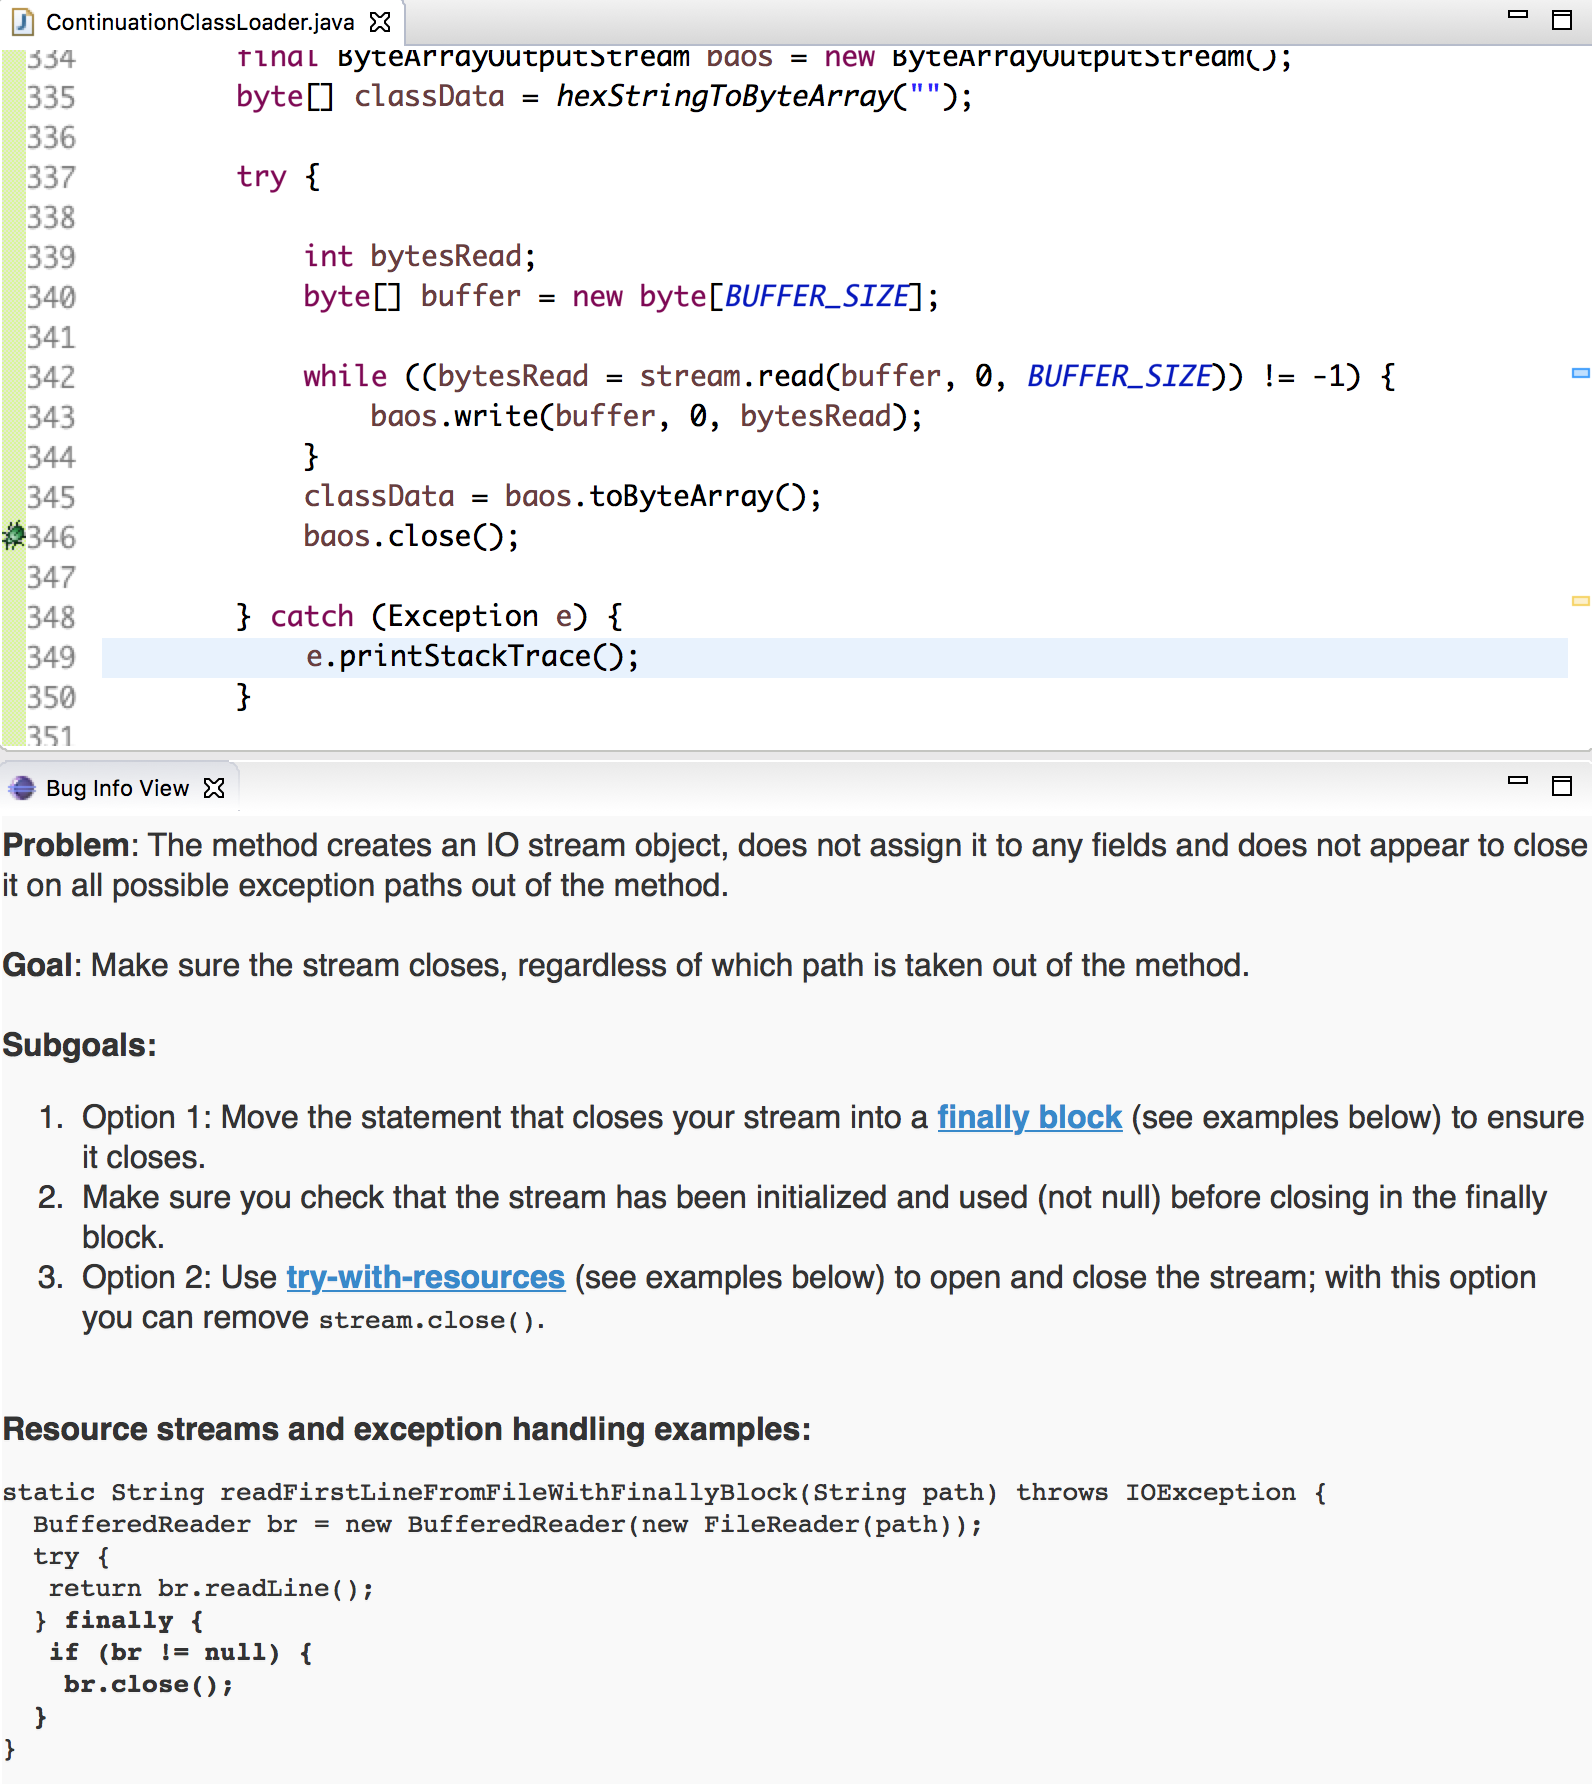
\includegraphics[width=5.5in]{Chapter-7/figs/novice}
	\caption{A notification modified for a developer classified as a novice in  exception handling.}
	\label{fig:novice}
\end{figure}

\begin{figure}
	\centering
	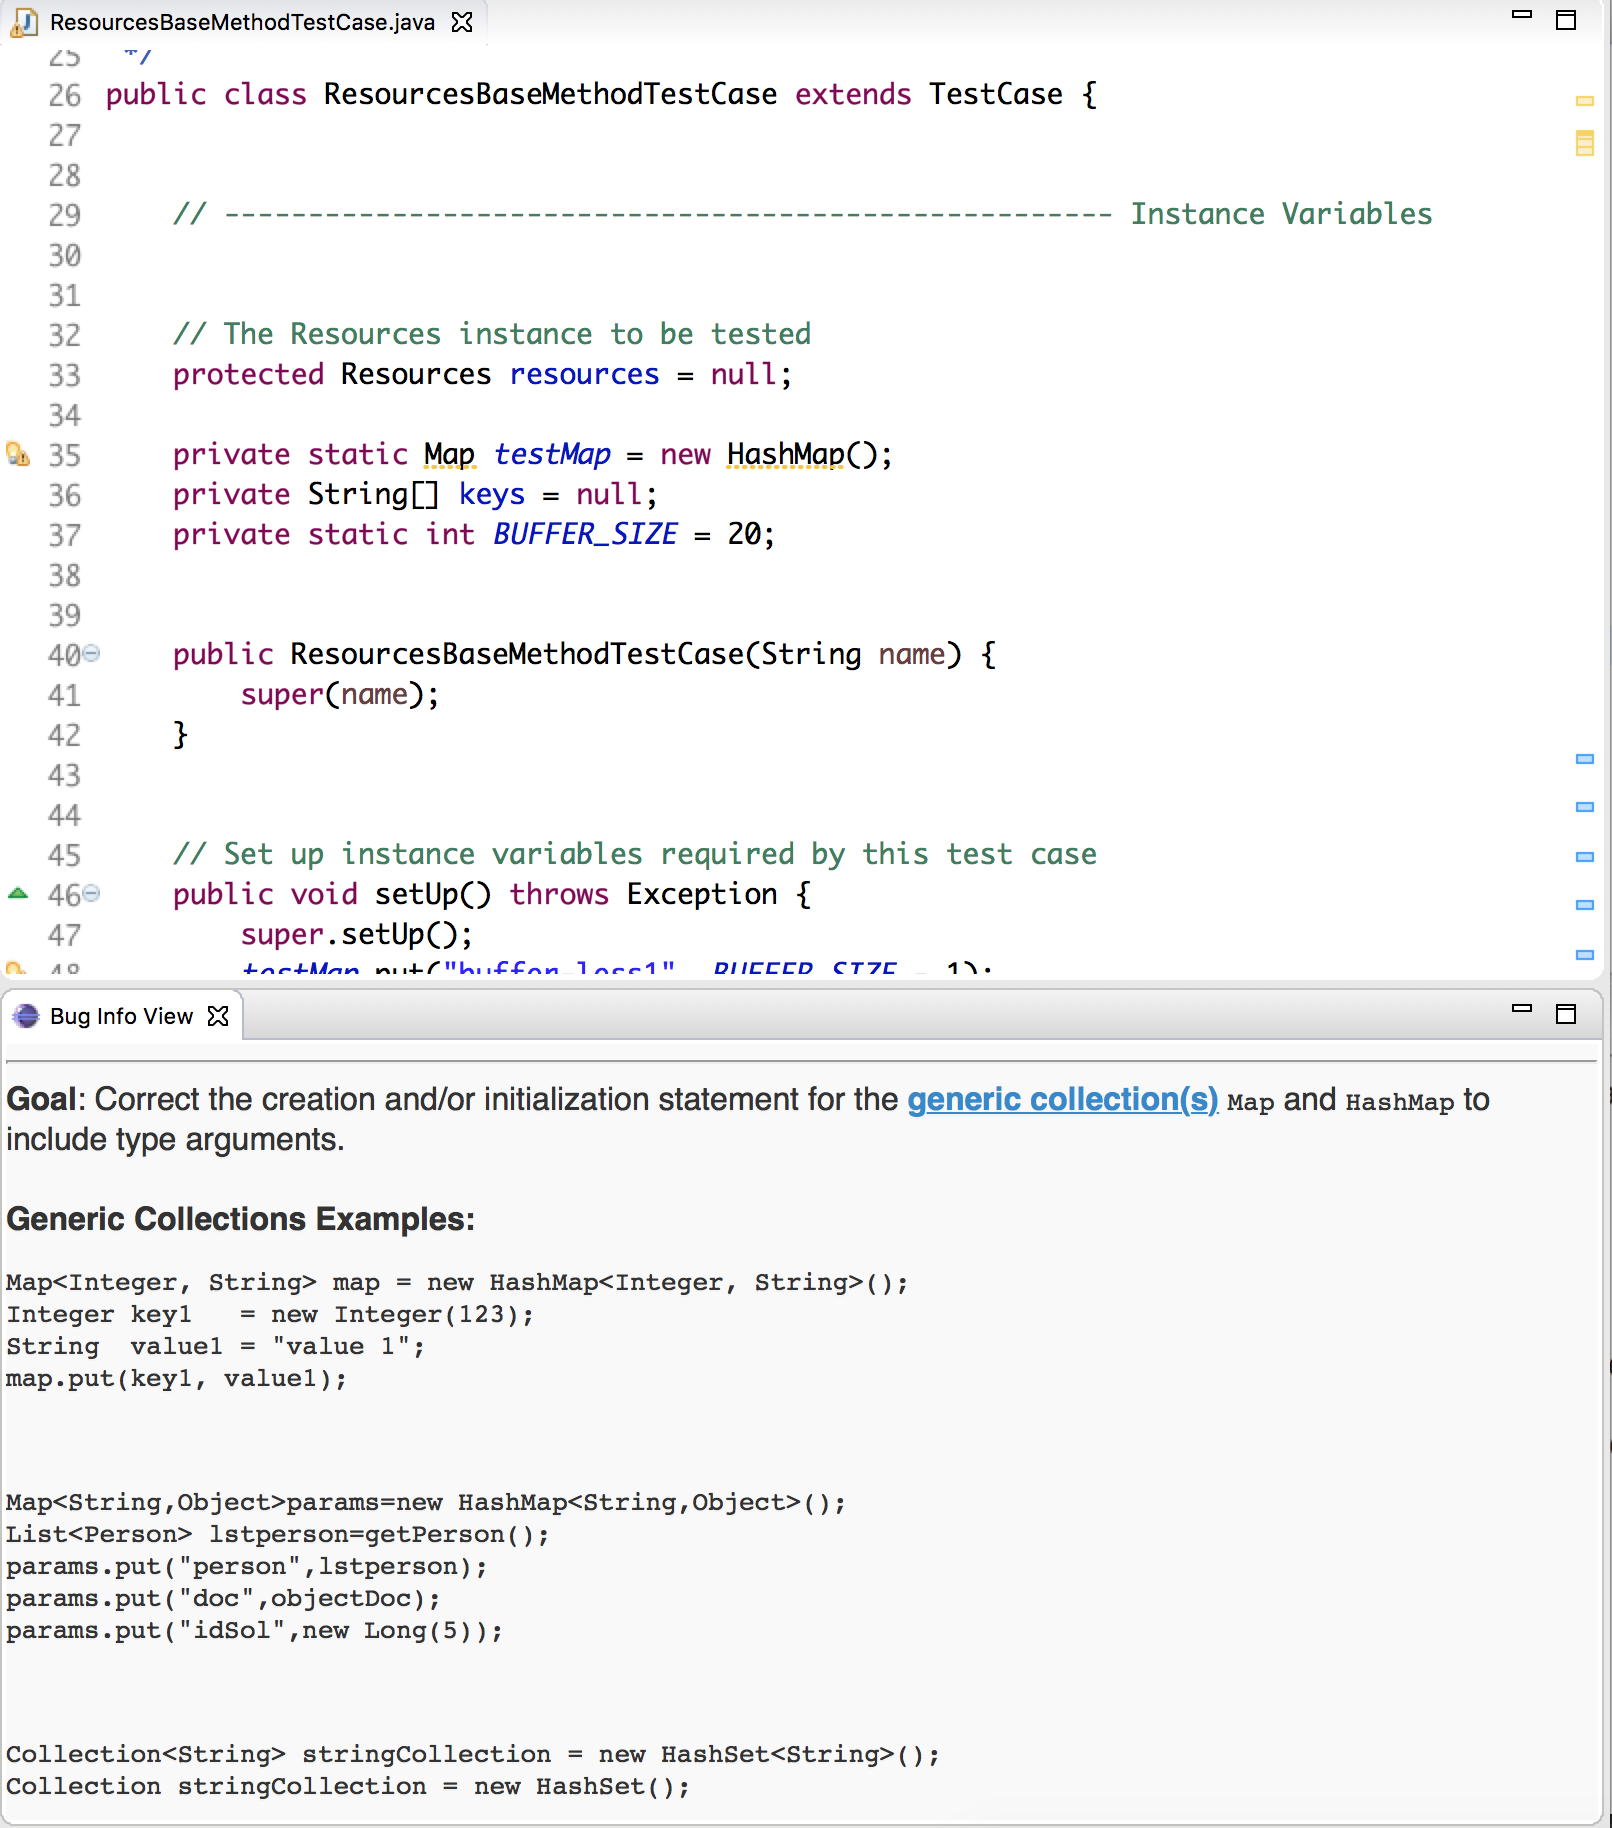
\includegraphics[width=5.5in]{Chapter-7/figs/expert}
	\caption{A notification modified for a developer classified as an expert in  generics.}
	\label{fig:expert}
\end{figure}

% provided insights into what examples I should include -- due technical and time limitations, used examples available online as-is. There exists technologies that can incorporate context-specificity into examples but evaluating availability of examples in notification rather than if they should be context specific.


% Further improved examples using attributes of good responses on StackOverflow~\cite{nasehi2012makes}:
% \item concise code
% \item use question context
% \item highlight important elements
% \item step-by-step -- this is general, based on research that suggests novices benefit more from step by step, part of novice notification design.
% \item links to extra resources
% \item multiple solutions -- why I included multiple examples when possible for each notification
% \item inline documentation
% \item solution \& API implications -- incorporated when necessary (give example?)


\subsection{Notification Selection}

Using the criteria outlined above, I modified 9 program analysis tool notifications from FindBugs and the Eclipse Java compiler, the same tools used in my previous study. I excluded ECLEmma to scope the current problem and solution to textual notifications. For each notification, I created a novice version and an expert version.

% how did I determine what defects to look for initially?
To determine the notifications for the user study, I attempted to find pre-existing defects in open source software. To narrow my search, I focused on defects that have been found to frequently appear in real world software projects~\cite{ayewah2010google}. 
I narrowed my search down to mature projects that were already Eclipse projects, could be relatively easily imported and compiled, and contains code snippets with libraries that are more likely to be familiar to developers.

% how did I find those defects and others to include?
Once I imported the projects, I analyzed the projects for compiler errors and warnings pertaining to the concepts of variables, exception handling, and generics.
I also ran FindBugs on each project to find defects pertaining to the concepts.
I went through the relevant notifications one by one to find code snippets that are not dependent on a large number of other classes and contain libraries and functionality that are familiar to the developer. The latter criteria was to mitigate the threat of developers looking at code that is not their own.

After analyzing a number of projects, I chose to go with the Java Collections library. I was able to find existing notifications from FindBugs and the compiler relevant to the concepts of interest. Because I needed enough notifications to populate my user study, I sometimes had to inject defects into the source code. When this was done, I chose code snippets where only minimal changes led to the introduction of the defect, error, or warning. Also, much of the code used in the library, and the functionality the library is written for, are familiar to developers regardless of their contributing to that code base.
The final set of defects used in the study can be found in Table~\ref{table:notifications}. For each notification in the table, I created a novice and expert version, for a total of 18 notifications.

\newcolumntype{g}{>{\columncolor{gray!40}}l}

\begin{table}[]
\centering
\caption{Notifications used in the user study.}
\label{table:notifications}
\begin{tabular}{lgg}
\toprule
\rowcolor{white}
                            & \textbf{Problem}                                                                                                         & \textbf{Tool} \\
\midrule
\rowcolor{white}
\textit{Variables}          & Unwritten field                                                                                                          & FindBugs      \\
                            & Unused field/parameter                                                                                                   & FindBugs      \\
    \rowcolor{white}
                            &   Incompatible types              & FindBugs               \\
\textit{Exception Handling} & Unhandled exception type                                                                                                 & Compiler      \\
\rowcolor{white}
                            & Method may fail to close stream on exception                                                                            & FindBugs      \\
                            & New exception not thrown                                                                                                      & FindBugs      \\
\rowcolor{white}
\textit{Generics}           & \begin{tabular}[c]{@{}l@{}}Inferred type argument(s) do not conform to the \\ bounds of the type variable(s)\end{tabular} & Compiler      \\
                            & \begin{tabular}[c]{@{}l@{}}Raw types: references to generic types should be \\ parameterized\end{tabular}               & Compiler      \\
\rowcolor{white}
                            & Cannot convert generic types                                                                                            & Compiler    \\
\bottomrule
\end{tabular}
\end{table}

\subsection{Adaptation Evaluation}

Once I had a set of modified notifications, I developed a wizard-of-oz plug-in to evaluate to evaluate H1, H2, and my RQ. This plug-in presents defects that have been augmented with modified notifications to participants. Below I outline the user study I designed to evaluate my hypotheses, which are:

\begin{itemize}
    \item [H\textsubscript{1}] Knowledge-based notifications can decrease the time required for notification resolution.
    \item [H\textsubscript{2}] Knowledge-based notifications can increase developer ability to resolve notifications.
    \item[RQ] Do developer adaptation preferences match expectations, based on existing literature?
\end{itemize}

% \subsubsection*{Participants}

Participants in this study were developers from academia and industry. 
I attempted to recruit participants using various sources, including departmental mailing lists, social media, and personal contacts.
I was able to obtain 14 user study participants, most of which I obtained through personal contacts in academia and industry.
All participants had prior experience with Java, Eclipse, and the Eclipse Java compiler. All but 4 participants had prior experience with FindBugs. 
Participants ranged from undergraduate students to professional developers with years of industry programming experience.

\subsubsection{Study Design}
% TODO rethink methodology labels (be consistent)

% quizzes
To evaluate knowledge-based notifications, I need to know when participants in  the study are looking at notifications that are aligned and misaligned with their knowledge. A notification is aligned with a participant's knowledge if the classification the notification was designed for matches the developer's classification. To determine developer classification, each participant completed concept inventories on the concepts relevant to the study. These are the same concept inventories used in Chapter~\ref{chap:experience}.

Each session lasted approximately 1 hour. In this hour, I asked participants to resolve the 9 defects selected. 
For the user studies I used two set-ups.
Rather than having all participants look at the same novice and expert notifications, I evaluated a novice and expert version for each notification across user studies. I alternated between two groups, each group consisting of a different subset of the 18 novice and expert notifications. In other words, all participants saw all 9 defects; but, for example, the novice notifications participants in Group 1 saw, another participant in Group 2 saw the expert version of that same notification.

% training exercise
At the beginning of each user study, I first briefed participants on what they would be doing. 
I also asked participants to rank their experience with Java, Eclipse, FindBugs, and the Eclipse Java compiler on a scale of 1 to 10 (1 being unfamiliar, 10 being extremely familiar). 
% TODO include some visual showing range of experience??

During this time, I also included instructions specifically regarding information they can and should be using to resolve the notifications and how to access it. Because I want to assess developers' ability to resolve defects based on the information provided in the notifications, I asked participants not to apply quick fixes. To reduce the temptation to use them, I disabled the information provided by compiler outside of the marker and squiggly underline. 

To re-enforce the process participants would be repeating during the study, I incorporated a training exercise into the beginning of the study. During the training exercise, participants did not have to resolve the notification but rather access and acknowledge the presence of the view that provides defect information.

After the training exercise, participants worked their way through each defect in their set of 9. I wanted to assess ability to resolve, therefore it was required that participants approach the problem as if they were going to resolve it. However, I let participants know that if they felt they would need more time than they had for the user study to explore and resolve the defect they could skip it. I did not want to force participants to work until they resolved the problem; the pilots I conducted suggested that after about an hour participants begin to feel fatigued and thereby less engaged in the study.

After participants resolved, or attempted to resolve, each notification, I debriefed with them to learn more about how they came to the solution they used. The goal of debriefing was to determine if the notification contributed to or hindered their ability to resolve the defect. This was also an opportunity to ask participants about experience with the individual defects. 

Some participants were distributed, therefore, I also had a remote set-up that I used to conduct user studies with remote participants. The remote set-up was similar to the local set-up; the only difference was that remote participants remotely controlled my computer to complete the user study while local participants physically used my computer. I recorded audio and the screen for all of the user studies in preparation for data analysis.

% TODO explain how I accounted for remote lag (determining when lag was affecting performance and remove time based on time wasted dealing with it)

\subsubsection{Data Analysis}

% Extract resolution times and correctness
The primary data point of interest was the time it took for participants to resolve each defect. 
Resolution of a defect for the sake of this study began when the participant opened and began to use the notification to work towards a resolution. For participants that attempted to resolve the defect without looking at the notification, time began when they either a) explored nearby code as if to determine the resolution or b) began fixing the defect if they did no exploring.

Along with time to resolve, I also collected data regarding the fixes participants selected to implement. For each defect, a fix was considered correct if it both compiled and would not cause new problems at runtime. For some defects, since they were pre-existing in the code base, I used Java best practices examples to determine the potential solutions. I also kept track of how many fixes participants attempted for each defect.

% Transcribe and analyze for qualitative (i.e. familiarity with notification) to support or better explain quantitative (resolution time) --> ??
% Extract notification preference by concept when existed ??
To supplement the quantitative data collected, and answer my RQ, I also analyzed the audio for statements made regarding the notifications and how well participants felt the notifications supported their resolution efforts.
For example, findings from the study discussed in Chapter~\ref{chap:theory} suggest familiarity with the notification can also affect developers' ability to interpret tool output. Therefore, this is something I want to keep track of as it may be able to help better explain the quantitative findings.

% one participant couldn't finish (timing)
All participants completed all three concept inventories necessary for data analysis, therefore I was able to use all the data provided by participants to evaluate my hypotheses.
One participant was unable to finish all the defects in the user study due to work obligations. Although he did not get to all 9 notifications, since he completed the inventories I analyzed data collected from the 7 he did complete.

To determine the significance between the differences calculated, I used R with RStudio~\cite{RSoftware} to run a two-sample unpaired t-test for set of aligned and misaligned values. I chose run a t-test because it can provide accurate results despite my small sample size. A t-test is also an  appropriate test for comparing averages across two samples that are different sizes.
I report the findins from these analyses in the next section.

\section{Adaptation Effectiveness}
% TODO rethink name?
Using the data from the user studies, I evaluated my hypotheses regarding developers' ability to resolve defects and their notification preferences.

\subsection{Resolving Adapted Notifications}

% TODO tables for all analyses run in R?

% table of mean resolution times (overall and by concept) -- include p-values

\begin{table}[]
\centering
\caption{Average time to resolve (seconds) aligned and misaligned notifications for each concept.}
\label{tab:concepts}
\begin{tabular}{lrrlrrl}
\toprule
                    & \textbf{\begin{tabular}[c]{@{}l@{}}Aligned \\ Novices\end{tabular}} & \textbf{\begin{tabular}[c]{@{}l@{}}Misaligned \\ Novices\end{tabular}} & \textbf{p-value}  & \textbf{\begin{tabular}[c]{@{}l@{}}Aligned \\ Experts\end{tabular}} & \textbf{\begin{tabular}[c]{@{}l@{}}Misaligned \\ Experts\end{tabular}} & \textbf{p-value}  \\
\midrule
\textbf{Variables}  & 156.1                                                               & 98.4                                                                   & \textit{0.192}   & 87.8                                                                & 88.7                                                                   & \textit{0.970}   \\
\textbf{Exceptions} & 46.9                                                                & 137                                                                    & \textit{0.019*} & 42.2                                                                & 79.1                                                                   & \textit{0.042*} \\
\textbf{Generics}   & 235.4                                                               & 249.8                                                                  & \textit{0.861}   & 237                                                                 & 341                                                                    & \textit{0.628}    \\
\hline
\textbf{Total}      & 148.25                                                              & 180.7                                                                  & \textit{0.446}   & 83                                                                  & 140.2                                                                  & \textit{0.130}  \\
\bottomrule
\end{tabular}
\end{table}

\newcolumntype{g}{>{\columncolor{gray!40}}l}

\begin{table}[]
\centering
\caption{Totals for aligned and misaligned defect resolution.}
\label{tab:total}
\begin{tabular}{lggggggg}
\toprule
\rowcolor{white}
                    &                                                                                 & \textbf{\begin{tabular}[c]{@{}l@{}}Aligned\\ Novices\end{tabular}} & \textbf{\begin{tabular}[c]{@{}l@{}}Misaligned\\ Novices\end{tabular}} & \textbf{p-value}  & \textbf{\begin{tabular}[c]{@{}l@{}}Aligned\\ Experts\end{tabular}} & \textbf{\begin{tabular}[c]{@{}l@{}}Misaligned\\ Experts\end{tabular}} & \textbf{p-value} \\
\midrule
\rowcolor{white}
\textit{Variables}  & \textbf{\begin{tabular}[c]{@{}l@{}}Total Defects \\ Attempted\end{tabular}}     & 9                                                                  & 6                                                                     & \textit{N/A}      & 14                                                                 & 11                                                                    & \textit{N/A}     \\
\rowcolor{white}
                    & \textbf{\% Resolved}                                                            & 78\%                                                               & 83\%                                                                  & \textit{0.8188}   & 100\%                                                              & 91\%                                                                  & \textit{0.2618}  \\
                    & \textbf{\begin{tabular}[c]{@{}l@{}}Avg. Attempts\\  to Resolution\end{tabular}} & 1                                                                  & 2                                                                     & 0.3558            & 2                                                                  & 2                                                                     & \textit{N/A}     \\
\rowcolor{white}
\textit{Exceptions} & \textbf{\begin{tabular}[c]{@{}l@{}}Total Defects \\ Attempted\end{tabular}}     & 13                                                                 & 8                                                                     & N/A               & 13                                                                 & 8                                                                     & \textit{N/A}     \\
                    & \textbf{\% Resolved}                                                            & 77\%                                                               & 100\%                                                                 & \textit{0.1529}   & 100\%                                                              & 100\%                                                                 & \textit{N/A}     \\
\rowcolor{white}
                    & \textbf{\begin{tabular}[c]{@{}l@{}}Avg. Attempts \\ to Resolution\end{tabular}} & 1                                                                  & 1                                                                     & \textit{N/A}      & 1                                                                  & 1                                                                     & \textit{N/A}     \\
\textit{Generics}   & \textbf{\begin{tabular}[c]{@{}l@{}}Total Defects \\ Attempted\end{tabular}}     & 15                                                                 & 18                                                                    & \textit{N/A}      & 3                                                                  & 6                                                                     & \textit{N/A}     \\
                    & \textbf{\% Resolved}                                                            & 73\%                                                               & 61\%                                                                  & \textit{0.4655}   & 100\%                                                              & 83\%                                                                  & \textit{0.4746}  \\
\rowcolor{white}
                    & \textbf{\begin{tabular}[c]{@{}l@{}}Avg. Attempts \\ to Resolution\end{tabular}} & 2                                                                  & 3                                                                     & 0.0950            & 1                                                                  & 1                                                                     & \textit{N/A}     \\
Total               & \textbf{\begin{tabular}[c]{@{}l@{}}Total Defects \\ Attempted\end{tabular}}     & 37                                                                 & 32                                                                    & \textit{N/A}      & 30                                                                 & 25                                                                    & \textit{N/A}     \\
\rowcolor{white}
                    & \textbf{\% Resolved}                                                            & 76\%                                                               & 75\%                                                                  & \textit{0.9238}   & 100\%                                                              & 92\%                                                                  & \textit{0.1179}  \\
                    & \textbf{\begin{tabular}[c]{@{}l@{}}Avg. Attempts \\ to Resolution\end{tabular}} & 1                                                                  & 3                                                                     & \textit{0.03703*} & 1                                                                  & 1                                                                     & \textit{N/A}    \\
\bottomrule
\end{tabular}
\end{table}


% \begin{table}[]
% \centering
% \caption{Totals for aligned and misaligned defect resolution.}
% \label{tab:total}
% \begin{tabular}{lll}
% \toprule
%                                                                              & \textbf{Aligned} & \textbf{Misaligned} \\
% \midrule                                                                            
% \textbf{\begin{tabular}[c]{@{}l@{}}Total Defects \\ Attempted\end{tabular}}  & 64               & 61                  \\
% \textbf{\% Resolved}                                                         & 86\%             & 82\%                \\
% \textbf{\% Not Resolved}                                                     & 14\%             & 18\%                \\
% \textbf{\begin{tabular}[c]{@{}l@{}}Avg. Time to \\ Resolve (s)\end{tabular}} & 124.9            & 154.1      \\
% \bottomrule
% \end{tabular}
% \end{table}


\subsubsection*{H\textsubscript{1} Findings}
Average resolution time in seconds of defects with aligned and misaligned notifications are shown in Table~\ref{tab:concepts} and Table~\ref{tab:total}. Table~\ref{tab:total} also reports the average attempts made to resolve notifications for each concept. 
Average attempts and resolution time for each participant are listed in Table~\ref{tab:resolved} and Table~\ref{tab:time}. 
I report a comparison of overall average resolution times and average resolution time by participant and by concept. For each concept, I observed the difference between averages for novices and experts. For each participant, I observed differences in their performance with aligned and misaligned notifications.

% significant time differences
Overall, it took participants less time to resolve the notifications aligned with their experience than notifications not aligned with their experience. 
The difference between resolution time was the largest for experts. 
This may have occurred because the notifications designed for novices provided more information to read, which some participants felt obligated to read regardless of needing the information.

Nine of the 14 participants spent less time on notifications aligned with their knowledge than they did on notifications not aligned with their knowledge.
For two participants, the aligned notifications significantly reduced the time to resolution (Table~\ref{tab:time}).
Also, despite there being more participants presented with aligned notifications (67) than misaligned notifications (57), participants took less time overall to resolve aligned notifications (231.25 seconds) than misaligned notifications (320.9 seconds). The difference was not significant, however, this may be due to the fact that I did not take into account other relevant factors, such as defect and notification experience, when determining developer concept knowledge classification.

Participants also took less time to resolve notifications aligned with their experience in
The concepts I evaluated include fundamental and nuanced concepts.
For exceptions and generics, the two more nuanced concepts, it took participants longer to resolve misaligned notifications.
It took participants significantly longer to resolve misaligned notifications on exception handling. 
This was the case for both novices and experts in exception handling.
With variables, the fundamental concept, it took participants more time to resolve the notifications aligned with their experience. 
This may be because 2 of the 3 notifications on variables I showed participants were a) associated with defects the participant was familiar with so they resolved the defect without reading much, if any, of the notification or b) notifications the participant would typically ignore.

The models I presented in Chapter~\ref{chap:experience} suggest generics may be the most nuanced of the three concepts. Following that theory, it makes sense that it took participants longer to resolve notifications on average with the generics notifications, regardless of which notification they saw.
Another explanation for this phenomenon is the participants' familiarity with the defect, as opposed to the notification, based on their prior experience.
Participants were generally more familiar with the defects related to variables and exceptions than the defects related to generics.

Familiarity with the defect affected the time it took for participants to resolve notifications.
This is related to my prior research that found notification familiarity affects notification resolution~\cite{johnson2016cross}. However, because I removed the familiar notifications, these findings suggest familiarity with the defect affects resolution time.
The affect of defect experience on resolution time was most evident with the concept of generics. Participants were most familiar with the compiler warning provided regarding raw types, therefore could all quickly provide a resolution regardless of the information provided.
Novices in generics credited their ability to recognize and resolve the problem to their prior experiences with the problem.
Participants were least familiar with the other two defects related to generics, leading to larger times attempting to understand and determine the best resolution. 


% This was not the case for experts in any other concept, which was to be expected given experts, according to existing research, are more likely to already have a plan for fixing the code~\cite{larkin1980expert, Wiedenbeck:1993:Mental}, regardless of the information provided. For some notifications, expert participants even noted skipping the subgoals completely when available because they already knew what to do. Most experts that the used subgoals noted using them for confirmation of their original plans.



\vspace{1em}

\fbox{%
	\parbox{0.9\linewidth}{%
		\noindent\textbf{\textit{These findings suggest that knowledge-based notifications do not always significantly decrease the time it takes for developers to resolve defects, but can significantly decrease the time it takes for developers to resolve defects.}}
	}%
}
\vspace{1em}

% \item [H\textsubscript{2}] Knowledge-based notifications can increase developer ability to resolve notifications


\begin{table}[]
\centering
\caption{Aligned and misaligned notifications resolved by each participant}
\label{tab:resolved}
\begin{tabular}{rrlcrrl}
\toprule
\multicolumn{3}{c}{\textbf{Aligned}}                                                                                                                                                                                                                                                 & \multicolumn{1}{l}{}                     & \multicolumn{3}{c}{\textbf{Misaligned}}                                                                                                                                                                                                                                               \\
\midrule
\multicolumn{1}{c}{\textbf{\begin{tabular}[c]{@{}c@{}}Notifications\\ Resolved\end{tabular}}} & \multicolumn{1}{c}{\textbf{\begin{tabular}[c]{@{}c@{}}Total\\ Notifications\end{tabular}}} & \multicolumn{1}{c}{\textbf{\begin{tabular}[c]{@{}c@{}}Percent\\ Resolved\end{tabular}}} & \multicolumn{1}{l}{\textbf{Participant}} & \multicolumn{1}{c}{\textbf{\begin{tabular}[c]{@{}c@{}}Notifications\\ Resolved\end{tabular}}} & \multicolumn{1}{c}{\textbf{\begin{tabular}[c]{@{}c@{}}Total\\ Notifications\end{tabular}}} & \multicolumn{1}{c}{\textbf{\begin{tabular}[c]{@{}c@{}}Percent \\ Resolved\end{tabular}}} \\
\hline
5                                                                                             & 5                                                                                          & 100\%                                                                                   & \textbf{P1}                              & 4                                                                                             & 4                                                                                          & 100\%                                                                                    \\
\rowcolor{yellow}
4                                                                                             & 4                                                                                          & 100\%                                                                                   & \textbf{P2}                              & 4                                                                                             & 6                                                                                          & 67\%                                                                                     \\
4                                                                                             & 5                                                                                          & 80\%                                                                                    & \textbf{P3}                              & 4                                                                                             & 4                                                                                          & 100\%                                                                                    \\
\rowcolor{yellow}
5                                                                                             & 6                                                                                          & 83\%                                                                                    & \textbf{P4}                              & 3                                                                                             & 4                                                                                          & 75\%                                                                                     \\
\rowcolor{yellow}
4                                                                                             & 5                                                                                          & 80\%                                                                                    & \textbf{P5}                              & 2                                                                                             & 4                                                                                          & 50\%                                                                                     \\
\rowcolor{yellow}
4                                                                                             & 5                                                                                          & 80\%                                                                                    & \textbf{P6}                              & 3                                                                                             & 4                                                                                          & 75\%                                                                                     \\
\rowcolor{yellow}
5                                                                                             & 5                                                                                          & 100\%                                                                                   & \textbf{P7}                              & 3                                                                                             & 4                                                                                          & 75\%                                                                                     \\
3                                                                                             & 5                                                                                          & 60\%                                                                                    & \textbf{P8}                              & 3                                                                                             & 4                                                                                          & 75\%                                                                                     \\
5                                                                                             & 5                                                                                          & 100\%                                                                                   & \textbf{P9}                              & 4                                                                                             & 4                                                                                          & 100\%                                                                                    \\
2                                                                                             & 3                                                                                          & 67\%                                                                                    & \textbf{P10}                             & 3                                                                                             & 4                                                                                          & 75\%                                                                                     \\
2                                                                                             & 3                                                                                          & 67\%                                                                                    & \textbf{P11}                             & 5                                                                                             & 6                                                                                          & 83\%                                                                                     \\
4                                                                                             & 4                                                                                          & 100\%                                                                                   & \textbf{P12}                             & 5                                                                                             & 5                                                                                          & 100\%                                                                                    \\
6                                                                                             & 6                                                                                          & 100\%                                                                                   & \textbf{P13}                             & 3                                                                                             & 3                                                                                          & 100\%                                                                                    \\
5                                                                                             & 6                                                                                          & 83\%                                                                                    & \textbf{P14}                             & 3                                                                                             & 3                                                                                          & 100\%     \\
\bottomrule
\end{tabular}
\end{table}

\begin{table}[]
\centering
\caption{Average resolution times (seconds) for aligned and misaligned notifications by participant.}
\label{tab:time}
\begin{tabular}{crrl}
\toprule
\textbf{Participant} & \multicolumn{1}{c}{\textbf{\begin{tabular}[c]{@{}c@{}}Average Time to Resolve\\ (Aligned)\end{tabular}}} & \multicolumn{1}{c}{\textbf{\begin{tabular}[c]{@{}c@{}}Average Time to Resolve\\ (Misaligned)\end{tabular}}} & \textbf{p-value}  \\
\midrule
P1                   & 147.6                                                                                                 & 215.25                                                                                                   & \textit{0.6018}   \\
P2                   & 120.5                                                                                                 & 77.25                                                                                                    & \textit{0.3245}   \\
P3                   & 238                                                                                                   & 338.75                                                                                                   & \textit{0.5994}   \\
P4                   & 172.8                                                                                                 & 179.3                                                                                                    & \textit{0.9607}   \\
P5                   & 103.75                                                                                                & 69                                                                                                       & \textit{0.4511}   \\
P6                   & 224.75                                                                                                & 110.33                                                                                                   & \textit{0.5086}   \\
P7                   & 124.2                                                                                                 & 75                                                                                                       & \textit{0.4537}   \\
P8                   & 108.33                                                                                                & 170.33                                                                                                   & \textit{0.3871}   \\
P9                   & 47.8                                                                                                  & 277.25                                                                                                   & \textit{0.1836}   \\
P10                  & 35                                                                                                    & 180.3                                                                                                    & \textit{0.0200*} \\
P11                  & 76                                                                                                    & 111.4                                                                                                    & \textit{0.4862}   \\
P12                  & 47.5                                                                                                  & 132.6                                                                                                    & \textit{0.0518*} \\
P13                  & 75.5                                                                                                  & 59.3                                                                                                     & \textit{0.6903}   \\
P14                  & 64.6                                                                                                  & 130.33                                                                                                   & \textit{0.4116}  \\
\bottomrule
\end{tabular}
\end{table}

\begin{table}[]
\centering
\caption{Average attempts made toward resolution by participant.}
\label{tab:attempts}
\begin{tabular}{crrl}
\toprule
\multicolumn{1}{c}{\textbf{Participant}} & \multicolumn{1}{c}{\textbf{\begin{tabular}[c]{@{}c@{}}Average Attempts to Resolution\\ (Aligned)\end{tabular}}} & \multicolumn{1}{c}{\textbf{\begin{tabular}[c]{@{}c@{}}Average Attempts to Resolution\\ (Misaligned)\end{tabular}}} & \multicolumn{1}{c}{\textbf{p-value}} \\
\midrule
P1                                       & 1.8                                                                                                          & 1.25                                                                                                            & \textit{0.388}                               \\
P2                                       & 1.5                                                                                                          & 1.3                                                                                                             & \textit{0.537}                                \\
P3                                       & 1.8                                                                                                          & 4.25                                                                                                            & \textit{0.298}                               \\
P4                                       & 1                                                                                                            & 2                                                                                                               & \textit{0.055* }                            \\
P5                                       & 1.4                                                                                                          & 1.75                                                                                                            & \textit{0.313}                               \\
P6                                       & 1.6                                                                                                          & 2.5                                                                                                             & \textit{0.809}                                \\
P7                                       & 1.6                                                                                                          & 1                                                                                                               & \textit{0.304}                               \\
P8                                       & 2.8                                                                                                          & 3.25                                                                                                            & \textit{0.374}                               \\
P9                                       & 1                                                                                                            & 2                                                                                                               & \textit{0.089}                              \\
P10                                      & 1.67                                                                                                         & 1.5                                                                                                             & \textit{0.495}                                \\
P11                                      & 76                                                                                                           & 114                                                                                                             & \textit{0.576 }                              \\
P12                                      & 1.25                                                                                                         & 2.4                                                                                                             & \textit{0.056*}                             \\
P13                                      & 1                                                                                                            & 1                                                                                                               & \textit{N/A}                                  \\
P14                                      & 1.83                                                                                                         & 3                                                                                                               & \textit{0.243}  
            \\
\bottomrule
\end{tabular}
\end{table}

\subsubsection*{H\textsubscript{2} Findings}

Overall, novices and experts in a given concept resolved a larger percentage of notifications aligned with their knowledge than notifications misaligned with their knowledge, as shown in Table~\ref{tab:resolved}.
The difference was the largest for experts (8\%), who resolved all of the aligned notifications.
This difference existed even though participants encountered more aligned notifications than misaligned.

Six of the 14 participants were able to resolve all the aligned notifications presented to them for each concept (Table~\ref{tab:resolved}. 
Two of the 6 participants resolved a higher percentage of aligned notifications than misaligned notifications.
The remaining four participants resolved 100\% of the defects presented to them, whether aligned or misaligned with their knowledge.

For 5 of the 14 participants, the aligned notifications led to resolution 5--30\% more often than misaligned notifications; these participants are highlighted in Table~\ref{tab:resolved}.
Four participants were able to resolve all the aligned and misaligned notifications presented to them, only one of which was an expert across all concepts.
Participants unable to resolve aligned notifications were often conceptual beginners. 
For many participants in this group, along with being a concept novice, they mentioned not having recent, or any, experience with the defect being presented. This combined with their lacking conceptual knowledge may have affected their ability to resolve these defects in the context and time limit of the study.

\vspace{1em}
\fbox{%
	\parbox{0.9\linewidth}{%
		\noindent\textbf{\textit{These findings suggest that knowledge-based notifications do not significantly increase developers' overall ability to resolve defects but can significantly decrease the attempts novices make to resolve notifications.}}
	}%
}
\vspace{1em}

\subsubsection*{H\textsubscript{3} Findings}

In order to resolve a defect, developers have to make changes to the source code. These changes, which in real software projects can lead to code churn, can affect the quality of the software~\cite{munson1998code,nagappan2005use}. The less code churn there is, the fewer opportunities there are for developers to introduce new defects. For novices in a given concept, knowledge-based notifications significantly decreased the attempts made to resolve the notifications. Some novices pointed out during this study that when they are unsure of a fix, they would try something and use any errors that follow to refine the solution.
Despite the proclamation of this strategy, it took novices in a given concept significantly fewer attempts to resolve notifications aligned with knowledge, averaging 1 attempt as opposed to the 3 attempts for misaligned notifications.
Experts took on average 1 attempt to resolve the defects in the study, regardless of alignment with their knowledge. 
These findings suggest aligned notifications were generally able to lead novices directly to a fix, where the misaligned notifications led to fishing expeditions for a fix.

\vspace{1em}
\fbox{%
	\parbox{0.9\linewidth}{%
		\noindent\textbf{\textit{These findings suggest that knowledge-based notifications do significantly decrease novice developers' attempts to resolve notifications but do not affect the number of expert developer attempts.}}
	}%
}
\vspace{1em}


The differences discovered in exploring H\textsubscript{1} -- H\textsubscript{3} are promising and suggestive, despite being in its infancy. This was a first run of user studies in a research area that has not been explicitly explored. Along with the quantitative data discussed above, I collected qualitative data regarding participants' notification preferences to further explore the usefulness of adapted notifications.

\subsection{Adaptation Preferences}

% RQ: do developer adaptation preferences match expectations, based on existing literature?

One explicit question I asked participants was their preference regarding the set of notifications provided for each concept. 
Eight participants selected a version they preferred for each concept. 
Six participants could not provide a best notification across concepts, typically due to their varying experience with the defects presented.

When the 8 participants were experts in a given concept they preferred the shorter, more concise notifications that were designed for them.
As suggested by prior research, experts typically already had plans for resolving the defects~\cite{larkin1980expert, Wiedenbeck:1993:Mental}, so they preferred some combination of the problem statement, goal statement, and examples provided.
One expert participant, who was classified as an expert in all concepts for the study, said she wished to have had the subgoals for all the notifications, but just as confirmation.

When the 8 participants were novices in a given concept, 90\% of the time they preferred the notifications designed for them, with subgoals that walk them through the problem and its solution. 
Four of the 8 mentioned preferring even moreso the solution-oriented subgoals (i.e. ``do this'' or ``try that'') rather than the exploration-oriented subgoals (i.e. ``find this'' or ``look at that'').
The handful of times participants did not prefer the notification designed for them noted preferring the expert notification because their prior experience with resolving the defect made the other information unnecessary.
All participants found the goal statements provided useful, especially when they were prescriptive (i.e. ``Add missing throw statement'').


For 6 participants, it was difficult to pick just one version for each concept; most often, it was when participants were expert in a given concept that they had more than one best notification.
In 8 instances, participants had varying levels of experience with the defects they had to resolve, which they stated made it difficult across notifications for primarily exceptions and generics. 
For these participants, the information they preferred depended on the defect they were trying to resolve. This coincides with my previous research that suggested defect knowledge also affects ability to understand and resolve notifications~\cite{johnson2016cross}.
% TODO example(s)?? quote(s)??


Inability to select a best notification may have also been affected by the grouping I selected for my two group set-up. 
For the purposes of this study, and based on existing research~\cite{mckeithen1981knowledge}, I grouped intermediate developers with experts. 
There was one participant who was classified as intermediate in generics, based on her score on the concept inventory, but because I chose a two option study design she was considered aligned with expert generics notifications in the study.
During her session, she constantly mentioned missing the subgoals when she did not have them. She noted that it was not that she always needed them but that it was nice to have them there when she did. She is also one of the experts that could not decide across concepts which notifications she preferred. 
It may be that there is a difference between intermediate expertise in software development and intermediate expertise in other STEM fields.



All participants found the availability of examples in the notification useful, as suggested by previous research~\cite{nasehi2012makes}; for many this was considered the most valuable information provided. 
% TODO can I say they resolved more often when examples short and closely matched??
Participants preferred short examples that closely matched the code they were looking at. 
Four participants noted being distracted by or having difficulty determining the useful parts of examples that were too long or too different from the code they were working in.
Similar to findings from~\cite{nasehi2012makes} on what makes a good example on StackOverflow, some participants wanted explanations with the code examples provided to ease integration into their own code.
Two participants requested the examples be partnered with the appropriate subgoal(s).



\vspace{0.5em}
\fbox{%
	\parbox{0.9\linewidth}{%
		\noindent\textbf{\textit{These findings suggest that some developer adaptation preferences match expectations, based on existing literature, and some do not.}}
	}%
}
\vspace{0.5em}

\subsection{Threats to Validity}
The findings from this study are promising and provide insights into the information needs of developers based on their conceptual knowledge. There are threats to the validity of this study that affected the results, which I discuss next.

\subsubsection{External Threats}
% only Java, only two tools
This user study evaluated modifying notifications from two tools amongst a number of tools that are available.
We also only focused on Java software projects.
However, the defects that we chose are reported by various tools and for different languages, increasing my confidence that these findings would generalize to other languages and tools.

% small data set
Finally, a common concern with empirical studies is the number of participants. Given the time-intensive nature of this study, I was only able to recruit 14 participants.This is on par with other similar studies~\cite{smith2015questions,Layman:2007:FaultFix}, though it may seem like a low number of participants. 
Along the same lines, there was a large number of participants classified as experts in exceptions which led to expert-heavy data for that concept; the same was true for generics novices.


\subsubsection{Internal Threats}
% technical things
I had to develop a plug-in that was capable of presenting the information I wanted to evaluate in a timely manner, therefore I was unable to implement a fully functional analysis tool. Rather I created a tool mock up that simulated the behaviors of a real tool. This introduced the potential for unexpected behavior and technical issues when running the application. I ran multiple pilots prior to the actual user studies to work out as many technical issues as possible so the set up was as realistic as possible.

% remote lag
Another technical issue that introduced a threat was the lag that came with conducting the remote interviews.This sometimes affected the time it took participants to resolve the defects.
For international participants, there also appeared to be a difference in the keyboard shortcuts typically used in Eclipse, which also affected some participants resolution time.

Due to time limitations, one participant was unable to address all the variables notifications. This also affected my results regarding H1 and H2. However, rather than throwing out this participant's data, I included it to show where value was provided in other notifications.

\subsubsection{Construct Threats}
% not their code
There also exists the threat of participants having to resolve defects in code that is not their own. This can affect the time it takes and how confident developers may feel about their fix. To mitigate this threat, I chose code snippets for each defect simple enough to be comprehensible in a short period of time but complex enough to still feel realistic.

% notification design based partially on problem solving in other STEM fields
I designed the notifications for this study using decades old research from Computer Science and other STEM fields. Having to start with research from other fields, and not specifically pertaining to notification design, may have affected the overall findings in particular. It is unclear whether proposed similarities between problem solving in other fields and Computer Science is still valid and apply to tool output. However, there are improvements these findings suggest can be made to potentially further improve communication between developers and their tools.

% experts sometimes didn't look at notification until after the fact so hard to determine in those situations if the notification was or was not useful
In some situations, participants could look at the code and recognize what the problem was or might be based on their prior experience. When this happened, some participants did not look at the notification provided prior to resolving; this was often the case with those classified as concept experts. This affected the ability to get feedback on what was and was not useful in the information provided. I attempted to mitigate this threat by asking those who did not use the notification to look at it after the fact for consistent debriefing.


\section{From ``Pipe Dream'' to Reality}
% TODO why was this endeavor worthwhile despite the results?
Findings from this study suggest that notifications modified and presented based on developer knowledge can be used to improve developer ability to understand and resolve defects. 
Even better, notifications that were modified to match developer knowledge sometimes reduced the time it took for resolution, suggesting the possibility of helping developers resolve defects more quickly.
Along with the general idea of adapting tool output to the developer's level of knowledge, these findings have other implications which I discuss next.

The theory presented in Chapter~\ref{chap:theory} suggested that lack of knowledge regarding a defect or notification pertaining to a defect can affect developers' ability to resolve them. The findings from this study support these findings and suggest that defect experience may play a greater role in action than could be realized theoretically. The data analyzed in this study suggests defect experience can sometimes make up for lacking conceptual knowledge, suggesting that concept knowledge coupled with defect knowledge may be more effective when determining developer classification. As I expand this area of my research, I plan to explore the feasibility of collecting and using information regarding defect resolution for improved knowledge classification.

% TODO novices need this....experts not a big deal...can we present them with anything? 


% general defect resolution information needs by expertise
Participants classified as novices in a given concept valued, and most often preferred, notifications that included subgoals that walked them through potential solutions to the defect. This aligns with existing research that suggests this is how novices solve problems~\cite{larkin1980expert}, which provides specific content to the notion of providing more information to novices. 
% When provided with only a goal and set of examples, novices typically took a large amount of time exploring various aspects of the code, and sometimes the web, with no obvious plan or direction.
For some concepts, there is more than a novice to expert progression.
In this study, there was a participant who wanted the subgoals to always be available.
One way to potentially account for concepts where there is an intermediate stage is to have subgoals always available but only expanded and visible initially for novices.
This would also support experts like some of the participants in this study that occasionally found value in the subgoals being present.
Participants classified as concept experts preferred notifications that provided concise feedback and confirmation on the problem in the code. 
These participants rarely went past, and typically preferred, the problem and goal statement when subgoals were available. The only time experts scrolled past the goal and problem statement was when they could not recall what the resolution looked like and wanted to see examples or to confirmation their process or resolution.

% importance of examples to experts and novices
% TODO importance of accurate examples??
Both concept novices and experts valued examples in the notifications, validating the decision to include them in both notifications. 
For novices, the examples often served as directions for how to implement a fix.
For experts that used the examples, they were used as confirmation of fixes they already had in mind or implemented.
% matching examples to context of defect (i.e. other examples from same code base) -- novices will copy from examples directly even if not exact fix
Novices and experts also agreed that if examples are going to be present, they should be similar to or match the context of the code the defect is attached to.
This would allow them to more quickly map what the example was suggested to the proper resolution for their code, something that research has found to be a desired trait~\cite{nasehi2012makes}.
Some participants suggested using general examples that are similar to the code with the defect, while others suggested using examples out of the code base they are in that match or are similar. 
Another example related suggestion made by concept novices was to break down the examples to match up with the subgoals.
Perhaps further exploration will find novices and experts have preferences regarding the kind of example presented to them.

 

\subsection{Challenges to Overcome}
% TODO do I need limitations too?

% how to get initial classification (talk about feedback loop here also)
One challenge that must be overcome to fully realize adaptive notifications and tools is the challenge of determining the first kind of notification to show developers, either novice or expert. I have shown we can use source code to classify developers based on their knowledge, but tools and environments would need access to both developers' source code and the attributes in developer's source code that matter for that concept. 

% how do tools get information for modification; along same lines, are there ways to ease/quicken process of modifying notifications (automatic rather than manual effort?)
Another challenge to overcome is how tools will retrieve information to populate the notifications. My user study used manually modified notifications; although this is useful for a study setting it is less useful, and less practical, to have to manually modify all the notifications a tool provides. Also, having to manually update existing  notifications might de-motivate toolsmiths from wanting to invest the time to do it. One area for further research is to explore the possibility of automating notification modification. One way this might be done is by borrowing from relevant StackOverflow posts that include steps to resolve similar defects.

% dealing with notifications that communicate about multiple concepts; what if developer expert in one of the concepts and novice in the others -- do these kinds of modifications look different?
In this proof-of-concept study, I chose notifications that communicate about one concept each. In reality, some notifications communicate about multiple concepts at a time.
To fully realize the potential of adapting notifications, there needs to be a way to determine all the concepts in a multi-concept notification and what information in the notification maps to which concept.
For example, what should tools do with multi-concept notifications when presenting to a developer who is an expert in one of the concepts but a novice in the rest?
Ideally, the tool would modify bits of information that communicate about the concepts the developer is less experienced with.

% determining best examples to present -- ideally there's a set that's best for novices and experts together rather than separately
Finally, findings from this study suggest examples are an important and valued part of developers' defect resolution process. 
Therefore, when examples are included, it is important to find the best, most relevant examples to display. 
The data collected from this study suggests the best examples for both novices and experts may be those that are similar to or match the code being fixed, are short, and highlight the important parts of the example if not able to be short.
Some participants mentioned wanting examples directly from the code base if possible.
More focused research should be done to better understand the examples developers find useful and more importantly how tools can access and display these examples.
